\chapter{Desenvolvimento de EVA}

\section{Apresentação do projeto}


A EVA (EV.G Virtual Assistant) é um \textit{chatbot} de domínio amplo que será capaz de interagir com os alunos vinculados ao EV.G na medida de suas necessidades.
Ela irá atender tais solicitações via mecanismo de conversação textual na plataforma de mensagens instantâneas chamada Telegram, no atendimento administrativo de uma secretaria acadêmica.

Por meio de EVA, os alunos vinculados ao EV.G poderão usufruir de várias funcionalidades.
Eles irão gerenciar seus cursos visualizando o andamento das inscrições, terão acesso ao catálogo unificado, calendário de turmas, histórico escolar e também serão auxiliados no processo de emissão de certificado. Tudo por meio de um acesso único e simplificado.

\section{Detalhamento dos requisitos de EVA}\label{especificacao-requisitos-eva}

Como dito \ref{cap:02:sec:05:projeto}, modelar o domínio de aplicação de um \textit{chatbot} é uma atividade de importante, pois, a partir desta atividade, pode se compreender a necessidade do sistema a ser construído, e também, definir os requisitos que o tornam útil.
É interessante deixar claro, que todo o processo de levantamento e validação dos requisitos foi realizado e entregue por parte da EV.G. Assim, não haverá nenhuma seção que aborde como se deu tal levantamento. Ao invés disso, os requisitos de EVA serão apenas detalhados nas subseções a seguir.

\subsection{Requisitos funcionais}

Na seção \ref{cap:02:sec:05:projeto:classificacao-requisitos}, foi explicado o que são os requisitos funcionais de um sistema. Abaixo, na Tabela \ref{tabela:tabela1}, estão listados os requisitos funcionais elencados para o sistema de EVA.

\begin{table}[htb]
\caption{Detalhamento de requisitos funcionais de EVA}
% \textsf{\caption{Especificação de requisitos funcionais de EVA}}
\label{tabela:tabela1}
% \center
% \footnotesize
\centering
\medskip
\begin{tabular}{|p{1.2cm}|p{3.5cm}|p{7.5cm}|}
  \hline
   \textbf{\#RF} & \textbf{Nome}  & \textbf{Descrição}  \\
    \hline
    RF01 & Conversação & Permitir que o usuário interaja com o \textit{chatbot} na língua portuguesa por meio de mensagens textuais em um \textit{messenger}. \\
    \hline
    RF02 & Compreensão & O \textit{chatbot} deve ser capaz de compreender o que o usuário solicita, através das mensagens textuais enviadas por ele, e tomar as devidas decisões para atende-lo. \\
    \hline
    RF03 & Autenticação & O \textit{chatbot} deve possuir uma forma de identificar o usuário que está solicitando acesso à aplicação. \\
   \hline
     RF04 & Visualizar o histórico escolar & O \textit{chatbot} deve informar ao usuário o seu histórico escolar completo caso seja solicitado por ele. \\
   \hline
    RF05 & Auxiliar na emissão de certificados & O \textit{chatbot} deve auxiliar o usuário no processo de emissão de certificados dos cursos concluídos por ele, caso seja solicitado por ele. \\
   \hline
    RF06 & Visualizar as inscrições de cursos abertos & O \textit{chatbot} deve exibir ao usuário quais inscrições de cursos que estão abertas, caso seja solicitado por ele. \\
   \hline
\end{tabular}
\end{table}

\subsection{Requisitos não funcionais}

Na seção \ref{cap:02:sec:05:projeto:classificacao-requisitos}, foi explicado o que são os requisitos não funcionais de um sistema. Abaixo, na Tabela \ref{tabela:tabela2}, estão listados os requisitos não funcionais elencados para o sistema de EVA.

\begin{table}[htb!]
\caption{Detalhamento de requisitos não funcionais de EVA}
\label{tabela:tabela2}
\center
\footnotesize
\begin{tabular}{|p{1.2cm}|p{3.5cm}|p{7.5cm}|}
  \hline
   \textbf{\#RNF} & \textbf{Nome}  & \textbf{Descrição}  \\
   \hline
    RNF01 & Disponibilidade & O sistema deve estar disponível continuamente (24 horas / 7 dias por semana). \\
   \hline
    RNF02 & Confidencialidade & O sistema deve garantir a visualização dos dados apenas pelo usuário associado. \\
   \hline
    RNF03 & Integridade & O sistema deve garantir que caso algum usuário falhe ao tentar se autenticar por três vezes consecutivas, bloqueie as tentativas de acesso dele durante 24 horas. \\
   \hline
   RNF04 & Portabilidade & O sistema deverá atender prioritariamente na plataforma de mensagens instantâneas Telegram. \\
   \hline
    RNF05 & Interoperabilidade & O sistema deverá se comunicar com algum serviço de Processamento de Linguagem Natural. \\
   \hline
    RNF06 & Implementação & O sistema deverá ser implementado utilizando a linguagem de programação Python. \\
   \hline
   
\end{tabular}
\end{table}\label{tabela:3}

\section{Casos de uso de EVA}\label{casos-de-uso-eva}

Na seção \ref{texto:especificando-com-casos-de-uso}, foi descrito o que são casos de uso e como eles normalmente são utilizados durante o projeto de um sistema. Elaborar os casos de uso permite definir quais funções de aplicação que o sistema deverá oferecer ao usuário~\cite{ReqJair}. Para a sua especificação, serão utilizados também alguns dos requisitos funcionais e não funcionais, que foram detalhados na seção \ref{especificacao-requisitos-eva}, para que se possa descrever as funcionalidades do sistema com ainda mais propriedade. Nas subseções a seguir, será realizado todo o processo de especificação e detalhamento dos casos de uso de EVA.

\subsection{Especificação dos atores}

Um ator é algo com comportamento, tal como uma pessoa (identificada por seu papel), um sistema ou uma organização~\cite{CraigLarman}. No que se diz respeito a EVA, foram identificados como atores o Visitante e o Aluno. Ambos poderão interagir com EVA, por meio de mensagens textuais, porém com as devidas restrições. É válido ressaltar, que a EVA não entra como ator, já que será o próprio sistema na qual está sendo modelando. Na Tabela \ref{tabela:tabela3} os atores são especificados.

\begin{table}[htb!]
\caption{Especificação dos atores do sistema de EVA}
\label{tabela:tabela3}
\center
\footnotesize
\begin{tabular}{|p{2cm}|p{3cm}|p{7.5cm}|}
  \hline
   \textbf{\#ATOR} & \textbf{Nome}  & \textbf{Descrição}  \\
   \hline
    ATOR01 & Visitante & Qualquer pessoa que interaja com EVA sem estar devidamente autenticado e identificado no sistema. \\
   \hline
    ATOR02 & Aluno & Qualquer pessoa que interaja com EVA e esteja devidamente autenticado e identificado no sistema. \\
   \hline
\end{tabular}
\end{table}


\subsection{Especificação dos casos de uso}

Como dito no começo desta seção, casos de uso permitem definir as funções de aplicação que o sistema deverá oferecer para o usuário. A partir dos requisitos funcionais identificados para EVA, foram extraídos os casos de uso especificados na Tabela \ref{tabela:tabela4}.

\begin{table}[htb!]
\caption{Especificação dos casos de uso de EVA}
\label{tabela:tabela4}
\center
\footnotesize
\begin{tabular}{|p{2cm}|p{3cm}|p{7.5cm}|}
  \hline
   \textbf{\#UC} & \textbf{Nome}  & \textbf{Descrição}  \\
   \hline
    UC01 & Dialogar com EVA & Os usuários do sistema poderão dialogar com EVA por meio de mensagens textuais, na língua portuguesa, através de um \textit{messenger}. A partir dessa funcionalidade, o usuário irá acessar todas as demais.\\
   \hline
    UC02 & Efetuar login & Autenticação de um usuário, permitindo que ele tenha acesso às funcionalidades restritas de EVA. \\
   \hline
    UC03 & Visualizar histórico escolar completo & O usuário poderá solicitar a visualização do histórico de todos os cursos que ele esteve matriculado no âmbito da EV.G. \\
   \hline
    UC04 & Receber auxílio na emissão de certificados & O usuário poderá solicitar auxilio para a emissão dos certificados dos cursos no qual ele finalizou no âmbito da EV.G. \\
   \hline
    UC05 & Visualizar inscrições de cursos abertos & O usuário poderá solicitar a visualização de todos os cursos na qual possui matricula ativa no âmbito da EV.G. \\
   \hline
    UC06 & Efetuar logout & O usuário deixará de estar autenticado no sistema. Com isso, ele volta a possuir acesso limitado às funcionalidades de EVA.\\
   \hline
\end{tabular}
\end{table}

\subsection{Diagrama de casos de uso}

Para descrever de forma visual e clara como se dará o vínculo entre os atores e os casos de uso identificados de EVA, foi criado um diagrama de casos de uso. Para a criação deste, foi utilizada a notação UML.

Na UML, os atores são representados como figuras ‘palito’. Cada caso de uso, que são as possíveis interações que poderão ser realizadas, é representada por uma elipse. As linhas fazem a ligação entre os atores e as interações. Na Figura \ref{cap:03:fig:diagrama}, está representado o diagrama de casos de uso de EVA.
\begin{figure}
    \centering
    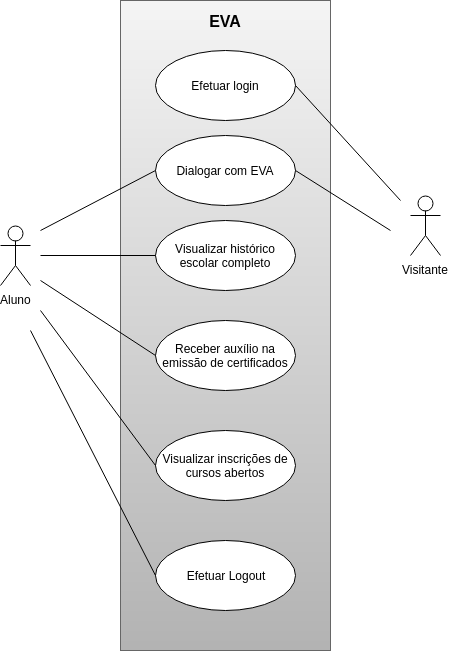
\includegraphics[width=0.3\linewidth]{src/imagens/CasoDeUsoEva.png}
    \caption{Fonte: Elaborado pelo autor (2018)}
    \label{cap:03:fig:diagrama}
\end{figure}

\subsection{Detalhamento dos casos de uso}

\subsubsection{UC01 - Dialogar com EVA}
\textbf{Descrição:} Este caso de uso especifica a ação principal de interação do usuário com o \textit{chatbot}, que é o diálogo. Por meio de mensagens textuais na língua portuguesa, o usuário poderá interagir com EVA e ter acesso à as suas funcionalidades. O nível de funcionalidades disponíveis para acesso do usuário, será determinada pelo fato dele estar autenticado ou não no sistema.

\begin{itemize}
    \item \textbf{Atores:}
        \begin{enumerate}
            \item ATOR01 - Visitante.
            \item ATOR02 - Aluno.
        \end{enumerate}
    \item \textbf{Requisitos funcionais:}
        \begin{enumerate}
            \item RF01 - Conversação.
            \item RF02 - Compreensão.
        \end{enumerate}
    \item \textbf{Requisitos não funcionais:}
        \begin{enumerate}
            \item RNF01 - Disponibilidade.
            \item RNF05 - Portabilidade.
            \item RNF05 - Interoperabilidade.
        \end{enumerate}
    \item \textbf{Fluxo básico:} 
        \begin{enumerate}
            \item O usuário envia uma mensagem textual para EVA.
            \item EVA irá consultar sua base de conhecimento para compreender o que o ator solicita.
            \item EVA responde ao usuário com base no que foi compreendido.
        \end{enumerate}
\end{itemize}

\subsubsection{UC02 - Efetuar login}
\textbf{Descrição:} Este caso de uso especifica a ação de autenticação no sistema, com o objetivo de identificar o aluno vinculado ao EV.G. A partir da autenticação, O aluno passará a receber auxilio personalizado e terá acesso aos recursos mais sofisticados de EVA. O usuário irá informar o seu CPF ou e-mail, EVA irá consultar na sua base de dados afim de verificar se o usuário de fato possui um vinculo com a EV.G, e então será determinado se há a possibilidade de ser realizada a autenticação ou não.

\begin{itemize}
    \item \textbf{Atores:}
        \begin{enumerate}
            \item ATOR01 - Visitante.
            \item ATOR02 - Aluno.
        \end{enumerate}
    \item \textbf{Pré-condições:}
        \begin{enumerate}
            \item O usuário deve possuir um vinculo com a EV.G.
        \end{enumerate}
    \item \textbf{Pós-condições:}
        \begin{enumerate}
            \item O usuário terá acesso às funcionalidades mais personalizadas de EVA.
        \end{enumerate}
    \item \textbf{Requisitos funcionais:}
        \begin{enumerate}
            \item RF01 - Conversação.
            \item RF02 - Compreensão.
            \item RF03 - Autenticação.
        \end{enumerate}
    \item \textbf{Requisitos não funcionais:}
        \begin{enumerate}
            \item RNF01 - Disponibilidade.
            \item RNF02 - Confidencialidade.
            \item RNF03 - Integridade.
            \item RNF05 - Interoperabilidade.
        \end{enumerate}
    \item \textbf{Fluxo básico:}
        \begin{enumerate}
            \item Ao início de uma conversação com EVA, ela irá solicitar que o usuário se identifique, para que ela possa lhe dar auxilio mais personalizado. Para isso, EVA irá solicitar que ele lhe informe o seu CPF ou e-mail cadastrados no EV.G.
            \item O usuário então irá informar o seu e-mail ou CPF.
            \item EVA irá verificar se o usuário está bloqueado no sistema.
            \item EVA irá verificar se o número de tentativas de autenticação chegaram ao valor limite, nesse caso, a três.
            \item EVA irá consultar em sua base de dados se as informações de fato conferem.
            \item O sistema então irá autenticar o usuário.
            \item EVA dá as boas vindas e informa ao usuário que a autenticação foi efetuada com sucesso.
            \item EVA apresenta as suas funcionalidades ao usuário e o convida a utilizar alguma.
        \end{enumerate}
    \item \textbf{Fluxo alternativo A:}
        \begin{enumerate}
            \item No Passo 5 do Fluxo Básico, após EVA consultar sua base de dados, foi visto que as informações não conferem.
            \item A contagem para o limite de tentativas de autenticação de um usuário é incrementada em um.
            \item EVA então informa ao usuário que os dados não conferem e pede para que ele informe o CPF ou o e-mail novamente.
            \item O fluxo retornar ao Passo 2 do Fluxo básico.
        \end{enumerate}
    \item \textbf{Fluxo alternativo B:}
        \begin{enumerate}
            \item No Passo 5 do Fluxo Básico, a mensagem textual enviada pelo usuário não aparenta ser nem algo parecido com CPF ou e-mail.
            \item EVA informa que ao usuário que ele precisa informar o CPF ou o e-mail para que ele possa se identificar, e assim, para que eles possam continuar dialogando.
            \item O fluxo retorna ao Passo 2 do Fluxo básico.
        \end{enumerate}
    \item \textbf{Fluxo alternativo C:}
        \begin{enumerate}
            \item No Passo 3 do Fluxo Básico, foi visto que o usuário está bloqueado no sistema.
            \item EVA informa que por questões de segurança, o usuário está bloqueado por um dia.
            \item EVA auxilia o usuário, que caso ele de fato ache que possui algum vinculo com a EV.G, que ele entre em contato através do e-mail da EVG.
            \item EVA informa o e-mail.
            \item EVA pede desculpa pelo transtorno.
        \end{enumerate}
    \item \textbf{Fluxo alternativo D:}
        \begin{enumerate}
            \item No Passo 4 do Fluxo Básico, foi visto que o usuário tentou se autenticar por três vezes sem sucesso.
            \item EVA bloqueia o usuário por um dia.
            \item EVA informa que por questões de segurança, o usuário está bloqueado por um dia.
            \item EVA auxilia o usuário, que caso ele de fato ache que possui um vinculo com a EV.G, que ele entre em contato através do e-mail da EVG.
            \item EVA informa o e-mail.
            \item EVA pede desculpa pelo transtorno.
        \end{enumerate}
\end{itemize}

\subsubsection{UC03 - Visualizar histórico escolar completo}
\textbf{Descrição:} Este caso de uso especifica a funcionalidade de EVA de pesquisar e informar o histórico escolar de um aluno vinculado ao EV.G. Para cada item identificado, EVA deve informar o nome do curso, a carga horária, o estado em que se encontra a matrícula do aluno e o estado de sua turma de ensino. 

\begin{itemize}
    \item \textbf{Atores:}
        \begin{enumerate}
            \item ATOR02 - Aluno.
        \end{enumerate}
    \item \textbf{Pré-condições:}
        \begin{enumerate}
            \item O usuário deve estar autenticado no sistema.
        \end{enumerate}
    \item \textbf{Requisitos funcionais:}
        \begin{enumerate}
            \item RF01 - Conversação.
            \item RF02 - Compreensão.
            \item RF04 - Visualizar histórico escolar.
        \end{enumerate}
    \item \textbf{Requisitos não funcionais:}
        \begin{enumerate}
            \item RNF01 - Disponibilidade.
            \item RNF02 - Confidencialidade.
            \item RNF04 - Portabilidade.
            \item RNF05 - Interoperabilidade.
        \end{enumerate}
    \item \textbf{Fluxo básico:}
        \begin{enumerate}
            \item O aluno envia uma mensagem textual para EVA solicitando o seu histórico escolar.
            \item EVA irá consultar sua base de conhecimento para compreender o que o aluno solicita.
            \item EVA irá consultar a base de dados da EV.G para pesquisar os dados escolares do aluno.
            \item EVA irá formatar os dados encontrados para serem exibidos ao aluno.
            \item EVA irá informar ao aluno o seu histórico escolar completo. Para cada item identificado, EVA deverá especificar os nome do curso, a cargas horária, o estado da matrícula do aluno e o estado da turma de ensino.
        \end{enumerate}
    \item \textbf{Fluxo alternativo A:}
        \begin{enumerate}
            \item No Passo 3 do Fluxo básico, foi constatado que o aluno não possui nenhuma matricula nos cursos da EV.G.
            \item EVA irá informar o aluno que ele não possui nenhuma matricula nos cursos da EV.G
            \item EVA irá sugerir ao aluno que ele visite o site da EV.G para ter acesso ao catálogo dos cursos oferecidos pela instituição.
        \end{enumerate}
\end{itemize}


\subsubsection{UC04 - Receber auxílio na emissão de certificados}
\textbf{Descrição:} Este caso de uso especifica a funcionalidade de EVA de auxiliar o aluno vinculado ao EV.G no processo de emissão de certificado. EVA irá pesquisar os cursos concluídos pelo aluno, e a partir destes, irá informar-lo quais procedimentos ele deverá realizar para emitir o certificado. Existem três situações possíveis para a emissão de certificados. O primeira situação, caso o curso tenha sido concluído no ano de 2015 para frente, EVA deve orientar o aluno a emitir o certificado no ambiente https://ava.enap.gov.br. O segundo, caso o curso tenha sido concluído entre os anos de 2013 a 2014, EVA deve orientar o aluno a emitir o certificado no ambiente https://moodle23.enap.gov.br. E o último, caso o curso tenha sido concluído antes do ano de 2013, EVA deverá orientar o aluno a enviar um e-mail para ead@enap.gov.br. Além das instruções para a emissão do certificado, para os itens de cada caso, EVA deverá informar o nome do curso e a carga horária.

\begin{itemize}
    \item \textbf{Atores:}
        \begin{enumerate}
            \item ATOR02 - Aluno.
        \end{enumerate}
    \item \textbf{Pré-condições:}
        \begin{enumerate}
            \item O usuário deve estar autenticado no sistema.
        \end{enumerate}
    \item \textbf{Requisitos funcionais:}
        \begin{enumerate}
            \item RF01 - Conversação.
            \item RF02 - Compreensão.
            \item RF05 - Auxiliar na emissão de certificados.
        \end{enumerate}
    \item \textbf{Requisitos não funcionais:}
        \begin{enumerate}
            \item RNF01 - Disponibilidade.
            \item RNF02 - Confidencialidade.
            \item RNF04 - Portabilidade.
            \item RNF05 - Interoperabilidade.
        \end{enumerate}
    \item \textbf{Fluxo básico:}
        \begin{enumerate}
            \item O aluno envia uma mensagem textual para EVA solicitando ajuda na emissão dos certificados.
            \item EVA irá consultar sua base de conhecimento para compreender o que o aluno solicita.
            \item EVA irá consultar a base de dados da EV.G para pesquisar os dados escolares do aluno.
            \item EVA irá formatar os dados encontrados para serem exibidos ao aluno.
            \item EVA irá auxiliar o aluno, com base no ano de conclusão dos cursos encontrados, quais procedimentos ele deverá realizar. Para cada situação, EVA informará o nome do curso e a carga horária de cada item.
        \end{enumerate}
    \item \textbf{Fluxo alternativo A:}
        \begin{enumerate}
            \item No Passo 3 do Fluxo principal, foi constatado que o aluno não concluiu nenhum curso da EV.G.
            \item EVA irá informar oa aluno que ele não concluiu nenhum curso da EV.G, logo, não tem como auxiliá-lo na emissão de certificados.
            \item EVA irá sugerir o aluno que ele visite o site da EV.G para ter acesso ao catálogo dos cursos oferecidos pela instituição.
        \end{enumerate}
\end{itemize}


\subsubsection{UC05 - Visualizar inscrições de cursos abertos}
\textbf{Descrição:} Este caso de uso especifica a funcionalidade de EVA de pesquisar e informar quais inscrições de cursos de um aluno vinculado ao EV.G que estão em aberto. Para cada item identificado, EVA deve informar o nome do curso, a carga horária, estado da matricula do aluno e o estado da turma. 

\begin{itemize}
    \item \textbf{Atores:}
        \begin{enumerate}
            \item ATOR02 - Aluno.
        \end{enumerate}
    \item \textbf{Pré-condições:}
        \begin{enumerate}
            \item O usuário deve estar autenticado no sistema.
        \end{enumerate}
    \item \textbf{Requisitos funcionais:}
        \begin{enumerate}
            \item RF01 - Conversação.
            \item RF02 - Compreensão.
            \item RF06 - Visualizar as inscrições de cursos abertos.
        \end{enumerate}
    \item \textbf{Requisitos não funcionais:}
        \begin{enumerate}
            \item RNF01 - Disponibilidade.
            \item RNF02 - Confidencialidade.
            \item RNF04 - Portabilidade.
            \item RNF05 - Interoperabilidade.
        \end{enumerate}
    \item \textbf{Fluxo básico:}
        \begin{enumerate}
            \item O aluno envia uma mensagem textual para EVA solicitando que deseja saber quais cursos que estão em aberto.
            \item EVA irá consultar sua base de conhecimento para compreender o que o aluno solicita.
            \item EVA irá consultar a base de dados da EV.G para pesquisar os dados escolares do aluno.
            \item EVA irá formatar os dados encontrados para serem exibidos ao aluno.
            \item EVA irá informar ao aluno quais cursos que estão em aberto. Para cada item identificado, EVA deverá especificar o nome do curso, o estado da matrícula, a carga horária e a situação da turma. 
        \end{enumerate}
        
    \item \textbf{Fluxo alternativo A:}
        \begin{enumerate}
            \item No Passo 3 do Fluxo principal, foi constatado que o aluno não possui inscrição em nenhum curso da EV.G.
            \item EVA irá informar ao aluno que ele não possui nenhuma inscrição nos cursos da EV.G.
            \item EVA irá sugerir o aluno que ele visite o site da EV.G para ter acesso ao catálogo dos cursos oferecidos pela instituição.
        \end{enumerate}
\end{itemize}

    
\subsubsection{UC06 - Efetuar logout}
\textbf{Descrição:} Este caso de uso especifica a funcionalidade onde o usuário deixará de estar autenticado no sistema.

\begin{itemize}
    \item \textbf{Atores:}
        \begin{enumerate}
            \item ATOR01 - Visitante.
            \item ATOR02 - Aluno.
        \end{enumerate}
    \item \textbf{Pré-condições:}
        \begin{enumerate}
            \item O usuário deve estar autenticado no sistema.
        \end{enumerate}
    \item \textbf{Pós-condições}:
        \begin{enumerate}
            \item O usuário deixará de estar autenticado no sistema, voltando a ter acesso limitado às funcionalidades de EVA.
        \end{enumerate}
    \item \textbf{Requisitos funcionais:}
        \begin{enumerate}
            \item RF01 - Conversação.
            \item RF02 - Compreensão.
        \end{enumerate}
    \item \textbf{Requisitos não funcionais:}
        \begin{enumerate}
            \item RNF01 - Disponibilidade.
            \item RNF02 - Confidencialidade.
            \item RNF04 - Portabilidade.
            \item RNF05 - Interoperabilidade.
        \end{enumerate}
    \item \textbf{Fluxo básico:}
        \begin{enumerate}
            \item O aluno envia uma mensagem textual para EVA solicitando que deseja efetuar o logout.
            \item EVA irá consultar sua base de conhecimento para compreender o que o aluno solicita.
            \item EVA irá desvincular o aluno de sua base de conhecimento.
            \item O aluno passa a ser um visitante.
            \item EVA irá informar de que o logout foi feito com sucesso.
        \end{enumerate}
\end{itemize}


\section{Modelagem dos diálogos de EVA}

Na seção \ref{texto:elaborando-dialogos} foi explicado como elaborar diálogos de um \textit{chatbot} a partir de cenários. Já na seção \ref{casos-de-uso-eva}, foram especificados e detalhados os casos de uso de EVA. Nesta seção, serão elaborados os diálogos, com base nos casos de uso de EVA, utilizando os cenários de cada um deles. É válido ressaltar, que existirão variações nas mensagens enviadas por EVA como resposta nos cenários especificados, porém, essas mensagens serão posteriormente cadastradas pela administração da EV.G.

\subsection{Cenários}

\subsubsection{Diálogo UC01 - Dialogar com EVA}

\begin{itemize}
    \item Suposição inicial:
    
    O usuário envia uma mensagem textual para EVA; EVA consulta sua base de conhecimento para compreender o que o ator solicita; EVA responde ao usuário.
    
    \begin{enumerate}
        \item \textbf{Usuário:} Olá, quem é você?
        \item \textbf{EVA:} Eu sou a EVA, a sua secretaria virtual da EVG. Eu posso pesquisar o seu histórico escolar, te auxiliar na emissão de certificados e também informar quais cursos estão em aberto!! Como posso lhe ser útil?
    \end{enumerate}
    
    \item O que pode dar errado:
    
    O usuário não autenticado solicitar o uso de alguma funcionalidade restrita de EVA.
    
        \begin{enumerate}
            \item \textbf{Usuário:} Informe o meu histórico escolar.
            \item \textbf{EVA:} Você ainda não está autenticado no nosso sistema. Por favor, se identifique me enviando seu e-mail ou CPF.
        \end{enumerate}
    
    O usuário solicitar algo que EVA não compreende.
    
        \begin{enumerate}
            \item \textbf{Usuário:} EVA, existe vida após a morte?
            \item \textbf{EVA:} Nossa, mil perdões, mas realmente eu não consegui entender o que você precisa.
        \end{enumerate}
\end{itemize}

\subsubsection{Diálogo UC02 - Efetuar login}

\begin{itemize}
    \item Suposição inicial: 
    
        EVA solicita que o usuário se identifique para que ela possa lhe dar auxilio mais personalizado; EVA solicita que o usuário informe o seu CPF ou o e-mail; o usuário informa o seu CPF ou e-mail; EVA informa que estará consultando as credenciais em seu banco de dados; EVA dá as boas vindas ao aluno.
        
        \begin{enumerate}
            \item \textbf{EVA:} Você ainda não está cadastrado no nosso sistema. Por favor, se identifique me enviando seu e-mail ou CPF.
            \item \textbf{Usuário:} test@evg.com
            \item \textbf{EVA:} Certo.. Aguarde alguns instantes enquanto eu faço a consulta no nosso banco de dados, está bem?
            \item \textbf{EVA:} Seja muito bem-vindo!! Eu sou a EVA, a sua assistente virtual do EV.G. Eu posso pesquisar o seu histórico escolar, te auxiliar na emissão de certificados e também informar a você quais cursos estão em aberto!! Fique a vontade, faça alguma pergunta.
        \end{enumerate}
    
    \item O que pode dar errado:
    
        As credenciais informadas pelo usuário não conferem.
        \begin{enumerate}
            \item \textbf{EVA:} Ops!! Parece que os dados informados não conferem. Por favor, tente novamente.
        \end{enumerate}
        
        O usuário envia uma mensagem textual que não é nada parecido com CPF ou e-mail.
        \begin{enumerate}
            \item \textbf{EVA:} Por favor, informe o seu e-mail ou o seu CPF. Caso você não tenha essas informações cadastradas, peço que entre em contato com a EV.G.
        \end{enumerate}
        
        O usuário tentou se autenticar por três vezes consecutivas sem sucesso.
        \begin{enumerate}
            \item \textbf{EVA:} Infelizmente, por motivos de segurança, estaremos bloqueando suas solicitações de registro por um dia. Caso você ache que os dados inseridos estão corretos, peço que você entre em contato com o EVG. Tente novamente amanhã, desculpe o transtorno.
        \end{enumerate}
        
        O usuário, já bloqueado, tenta se autenticar novamente.
        \begin{enumerate}
            \item \textbf{EVA:} Por motivos de segurança, você está bloqueado por um dia. Caso você ache que os dados inseridos anteriormente estejam corretos, peço que você entre em contato com o EVG. Tente novamente amanhã, desculpe o transtorno.
        \end{enumerate}
    
\end{itemize}

\subsubsection{Diálogo UC03 - Visualizar histórico escolar completo}

\begin{itemize}
    \item Suposição inicial:
    
        O aluno envia uma mensagem textual para EVA solicitando o seu histórico escolar; EVA irá consultar a base de dados da EV.G para pesquisar os dados do histórico do aluno; EVA se desculpa por ter deixado o aluno esperando; EVA informa o histórico escolar do aluno.
        
        \begin{enumerate}
            \item \textbf{Aluno:} EVA, gostaria de verificar meu histórico escolar, por favor.
            \item \textbf{EVA:} Só um segundo.
            \item \textbf{EVA:} Desculpe a demora! Aqui estão os dados que você solicitou.
            \item \textbf{EVA:} Curso: Informática básica; \\
            Carga horária: 70 horas; \\
            Situação da matrícula: Concluído; \\
            Situação da turma: Finalizada;\\ \ldots
        \end{enumerate}
    
    \item O que pode dar errado:
    
        O usuário não possui nenhuma inscrição nos cursos da EV.G.
        
        \begin{enumerate}
            \item \textbf{EVA:} Parece que você não tem nenhuma informação a ser exibida.
            \item \textbf{EVA:} Porque você não inicia um curso na nossa plataforma? Para ter acesso ao catálogo dos cursos da EV.G, acesse: https://evg.gov.br/catalogo.
\end{enumerate}
    
    \item Estado do sistema na conclusão:
    
        Após atender o aluno, EVA irá perguntar se o mesmo deseja mais alguma coisa.
        
        \begin{enumerate}
            \item \textbf{EVA:} Deseja mais alguma coisa?
        \end{enumerate}
    \end{itemize}

\subsubsection{Diálogo UC04 - Receber auxílio na emissão de certificados}

\begin{itemize}
    \item Suposição inicial:
    
        O aluno envia uma mensagem textual para EVA solicitando auxilio na emissão de certificados; EVA irá consultar a base de dados da EV.G para pesquisar os dados dos cursos concluídos do aluno; EVA se desculpa por ter deixado o aluno esperando; EVA auxilia o aluno no processo de emissão de certificado.
        
        \begin{enumerate}
            \item \textbf{Aluno:} Eu gostaria de auxílio na emissão dos meus certificados, por favor.
            \item \textbf{EVA:} Só um segundo.
            \item \textbf{EVA:} Desculpe a demora! Aqui estão os dados que você solicitou.
            \item \textbf{EVA:} Você finalizou o(s) seguinte(s) curso(s) no período de 2015 em diante: Empreendedorismo (CH - 50 horas) e Gestão de negócios (CH - 60 horas). \\
            Para emitir o certificado de algum curso relacionado acima, acesse: https://ava.enap.gov.br.
            \item \textbf{EVA:} Você finalizou o(s) seguinte(s) curso(s) no período de 2013 a 2014: Introdução a vigilância sanitária (CH - 60 horas). \\
            Para emitir o certificado de algum curso relacionado acima, acesse: https://moodle23.enap.gov.br/.
            \item \textbf{EVA:} Você finalizou o(s) seguinte(s) curso(s) no período anterior a 2013: Federalismo fiscal no Brasil (CH - 50 horas). \\
            Para emitir o certificado de algum curso relacionado acima, envie um e-mail para 'ead@enap.gov.br', com o título do curso que você deseja emitir o certificado, o seu nome e CPF.
        \end{enumerate}
    
    \item O que pode dar errado:
    
        O usuário não possui nenhuma inscrição nos cursos da EV.G.
        
        \begin{enumerate}
            \item \textbf{EVA:} Parece que você não tem nenhuma informação a ser exibida.
            \item \textbf{EVA:} Porque você não inicia um curso na nossa plataforma? Para ter acesso ao catálogo dos cursos da EV.G, acesse: https://evg.gov.br/catalogo.
        \end{enumerate}
    
    \item Estado do sistema na conclusão:
    
        Após atender o aluno, EVA irá perguntar se o mesmo deseja mais alguma coisa.
        
        \begin{enumerate}
            \item \textbf{EVA:} Deseja mais alguma coisa?
        \end{enumerate}
\end{itemize}


\subsubsection{Diálogo UC05 - Visualizar inscrições de cursos abertos}

\begin{itemize}
    \item Suposição inicial:
    
        O aluno envia uma mensagem textual para EVA solicitando a visualização dos cursos em aberto; EVA irá consultar a base de dados da EV.G para pesquisar os dados dos cursos que estão em aberto do aluno; EVA se desculpa por ter deixado o aluno esperando; EVA informa o aluno quais são os seus cursos em aberto.
        
        \begin{enumerate}
            \item \textbf{Aluno:}
            \item \textbf{EVA:} Só um segundo.
            \item \textbf{EVA:} Desculpe a demora! Aqui estão os dados que você solicitou
            \item \textbf{EVA:} Curso: Ética e Serviço público; \\
            Carga horária: 20 horas; \\
            Situação da matrícula: Em andamento; \\
            Situação da turma: Aberto;\\ \ldots
        \end{enumerate}
    
    \item O que pode dar errado:
    
    O usuário não possui nenhuma inscrição nos cursos da EV.G.
    
        \begin{enumerate}
            \item \textbf{EVA:} Parece que você não tem nenhuma informação a ser exibida.
            \item \textbf{EVA:} Porque você não inicia um curso na nossa plataforma? Para ter acesso ao catálogo dos cursos da EV.G, acesse: https://evg.gov.br/catalogo.
        \end{enumerate}
    
    \item Estado do sistema na conclusão:
    
        Após atender o aluno, EVA irá perguntar se o mesmo deseja mais alguma coisa.
        
        \begin{enumerate}
            \item \textbf{EVA:} Deseja mais alguma coisa?
        \end{enumerate}
    
\end{itemize}

\subsubsection{Diálogo UC06 - Efetuar logout}

\begin{itemize}
    \item Suposição inicial:
    
        O aluno envia uma mensagem textual para EVA solicitando que deseja efetuar o logout no sistema.
        
        \begin{enumerate}
            \item \textbf{Aluno:} EVA, gostaria de efetuar o logout.
            \item \textbf{EVA:} Só um segundo.
            \item \textbf{EVA:} O logout foi efetuado com sucesso. Lembre-se, sempre que desejar eu estarei por aqui, basta apenas informar o seu e-mail ou CPF. Até logo!
        \end{enumerate}
    
    \item Estado do sistema na conclusão:
    
        O aluno deixa de estar autenticado no sistema de EVA.
\end{itemize}


\section{Arquitetura de EVA}

Na seção ~\ref{chatbot:dev}, foram exemplificadas as duas formas utilizadas no desenvolvimento de \textit{chatbots}, que são utilizando plataformas de \textit{chatbots} ou não. Para o desenvolvimento de EVA, foi optado pela não utilização dessas plataformas. Assim, será necessário que haja uma explicação a cerca das tecnologias utilizadas, e também, da arquitetura escolhida para a sua criação.

No que diz respeito a arquitetura de EVA, pode-se dizer que esta consiste em duas partes principais: a API e o \textit{chatbot} propriamente dito. Nas subseções abaixo, serão detalhados as tecnologias que irão compor todo o sistema de EVA e também detalhes sobre a implementação.

\subsection{Tecnologias}

Nesta subseção, serão detalhadas as principais tecnologias utilizadas em todo o desenvolvimento de EVA, tanto para a criação da API, quanto para o \textit{chatbot} propriamente dito.

\subsubsection{Python}

A linguagem de programação base de todo o sistema de EVA, é o Python. Numa breve descrição sobre a linguagem, pode-se citar que ela é multi paradigma, suportando o paradigma orientado a objetos, imperativo, funcional e procedural; possui também tipagem dinâmica, onde não se é necessário declarações dos tipos de dados que serão utilizados durante a programação; e também, por possuir diversos frameworks que facilitam no desenvolvimento de aplicações, no qual, para o desenvolvimento de EVA, serão utilizados dois destes.

A escolha do Python como linguagem base para o desenvolvimento de EVA, se deu a partir da experiência do autor com a mesma, e também, pela liberdade de escolha por parte da EV.G.

\subsubsection{Django}

Para a implementação da API, que será detalhada mais adiante, foi utilizado o framework Django.

\subsubsection{Wit.ai}

Por se tratar de um \textit{chatbot} de domínio amplo, o sistema de EVA necessariamente precisa utilizar de algum recurso de IA, como abordado na seção \ref{cap:02:sec:01:sub:02:bot-dominio}. Para isso, pode-se utilizar técnicas de Aprendizagem de Máquina, descrita na seção \ref{cap:02:sec:02:sub:machine-learning} ou PLN, descrita na seção \ref{cap:02:sec:02:sub:pln}.
Para o desenvolvimento de EVA, fará-se uso da técnica de PLN. Para isso, serão utilizados os serviços oferecidos pelo Wit.ai.

 Wit.ai é uma plataforma de desenvolvimento de PLN gratuita que transforma a linguagem natural (fala ou escrita) em dados estruturados. É válido ressaltar também, que o Wit.ai oferece uma biblioteca para a utilização dos seus serviços em Python, sendo este, um dos principais motivos para a sua escolha.

\subsubsection{Telegram-bot-api}


\subsection{Arquitetura da API}

\subsection{Arquitetura do \textit{chatbot}}